% 3456789012345678901234567890123456789012345678901234567890123456789012
%        1         2         3         4         5         6         7
%
% Format: LaTeX
%
% For information about this file, contact the author by email at
% joe.loughry@lmco.com, or by telephone: +1 303 224 9618 (home), or
% +1 303 203 2067 (pager) or +1 303 203 2067 (office).  The time zone is
% GMT minus 7 hours.
%
% 20070420 (rjl) derived from standard skeleton and Makefile
%

% \documentclass[12pt]{article}

\documentclass{article}
\usepackage{url,amsmath,epic,eepic,epsfig}

% \raggedbottom
% \raggedright

\title{Notes on the Centroid of a Shield}

\author{J.\ Loughry}

% \date{}
\date{2007 April 20}

\begin{document}
\maketitle

\begin{abstract}

The region to be analyzed is defined by a rectangular area one unit high
and three units wide, surmounting an approximately triangular bottom area
delineated by a pair of circular arcs of radius three.  The centroid is a
point along the axis of symmetry corresponding to the center of mass of a
planar lamina of uniform density.

\end{abstract}

\section{Introduction}

The classical shape of the heraldic shield (called a ``heater'' shield because
the shape resembles an old-fashioned flatiron\footnote{The name is said to
date from Victorian times\cite{heater-shield-victorian-curators},
but I have not yet found a primary source to back up this assertion.})
is defined by a rectangular top region one unit high
by three wide, surmounting an approximately
triangular bottom region delineated by a pair of circular arcs of radius
three \cite{classical_heraldry}.

\begin{figure}[htbp]
  \centering
  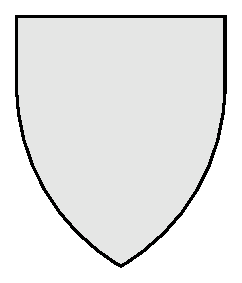
\epsfig{file=shield.eps, scale=0.5}
  \caption{EPS figure.}
  \label{figure:eps-figure}
\end{figure}

To properly place charges on the field, it is necessary to locate the ``middle''
of the shield.  Clearly, this lies along the axis of symmetry, but where,
exactly, along a top-to-bottom line?  Arguably the best choice is the centroid,
corresponding to the center of gravity of a physical piece of armor \cite{apostol:finding-centroids}.

\section{Constructing the Shape}

To draw a shield $R$ units wide, begin with a horizontal line segment from
$(-\frac{1}{2}R,-\frac{1}{3}R)$ to $(\frac{1}{2}R,\frac{1}{3}R)$.  Draw a
vertical line segment of length $\frac{1}{3}R$ from
$(-\frac{1}{2}R,0)$ to $(-\frac{1}{2}R,\frac{1}{3}R)$ and
another from $(\frac{1}{2}R,0)$ to $(\frac{1}{2}R,\frac{1}{3}R)$.  Draw an arc
centered at $(-\frac{1}{2}R,0)$ with radius $R$ through an angle from $0$ to
$-\frac{\pi}{3}$, and another arc centered at $(\frac{1}{2}R,0)$ with radius $R$ from
$\pi$ to $\frac{3\pi}{2}$ (Figure \ref{figure:Construction}).

The angle $\alpha = \frac{\pi}{3}$.  The width of the shield is $R$ and the bottom
is the point $(0,-\frac{1}{2}\sqrt{3R^2})$.

\begin{figure}[htbp]
  \setlength{\unitlength}{6mm}
  \begin{center}
    % offset the origin to the center of the picture frame
    % \begin{picture}(width,height)(x-offset,y-offset)
    \begin{picture}(6,7)(-3,-4)

		% coordinate axes (y-minus is longer)
		\put(0,0){\vector(0,1){2.2}} \put(-0.1,2.4){$y$}
		\put(0,0){\vector(0,-1){3.5}}
		\put(0,0){\vector(1,0){2.5}} \put(2.6,-0.1){$x$}
		\put(0,0){\vector(-1,0){2.5}}

		% rectangular upper portion of shield, centered on origin.
		\put(-1.5,1){\line(1,0){3}}
		\put(-1.5,1){\line(0,-1){1}}
		\put(1.5,1){\line(0,-1){1}}

		\put(-0.5,1){\line(0,-1){1}}
		\put(0.5,1){\line(0,-1){1}}

		% bottom part of shield
      \put(-1.5,0){\arc{6}{-0.2}{1.2}}
		\dashline{0.1}(-1.5,0)(0,-2.59)
		\put(-1.5,0){\arc{1}{0}{1.0472}}
		\put(-1,-0.5){$\alpha$}

	\end{picture}
  \end{center}
  \caption{Construction}
  \label{figure:Construction}
\end{figure}

The arcs intersect at a point $(0,-\frac{1}{2}\sqrt{3R^2})$ which can be found
by the circle formula $ (x-h)^2 + (y-k)^2 = R^2 $ with $h=-\frac{1}{2}R$ and $k=0$.
Then,
  $$(x+\frac{1}{2}R)^2 = y^2 = R^2 $$
  $$ x^2 + Rx + \frac{1}{4}R^2 + y^2 = R^2 $$
  $$ y^2 = R^2 - x^2 - Rx - \frac{1}{4}R^2 $$
  $$ y^2 = -z^2 -Rx + \frac{3}{4}R^2 $$
and by the quadratic formula\ldots

The $y$-intercept is $-\frac{1}{2}\sqrt{3R^2}$.

The width of the shield is $R$.  The height of the shield is
$\frac{1}{3}R + \frac{1}{2}\sqrt{3R^2}$.

\section{Finding the Centroid}

The centroid can be found most easily by decomposing the shield
into pieces: the top rectangle, two triangles, and two circular segments
(themselves decomposed into a circular sector and its inscribed triangle).
For each piece, we need to find the centroid and area of that piece.

\subsubsection{Rectangle}

The centroid of the rectangular top section is located at the intersection of
the diagonals: $(\bar{x}_r,\bar{y}_r) = (0,\frac{R}{2})$.  The area of the
rectangle $A_r = R$.

\subsubsection{Triangles}

The centroid of a right triangle lies one-third of way along the sides
from the central vertex of the right angle (cite!).  The height
of the triangle is $h = \frac{\sqrt{3R^2}}{2}$ and its base is $b = \frac{R}{2}$;
therefore $(\bar{x}_t,\bar{y}_t) = (\frac{R}{6},\frac{\sqrt{3R^2}}{6})$
and
  $A_t = \frac{1}{2}R\cdot\frac{\sqrt{3R^2}}{2}
       = \frac{R\sqrt{3R^2}}{4}
		 = \frac{R^2\sqrt{3}}{4}
		 = \frac{1}{4}R^2\sqrt{3}
		 = \frac{\sqrt{3}}{4}R^2$.

\subsection{Circular Segments}

The area of the circular segment is equal to the area of the circular sector
minus the area of the inscribed triangle.  The sector angle $\alpha = \frac{\pi}{3}$
and the area of the sector is $\pi R^2 \cdot \frac{\alpha}{2\pi} = \frac{1}{6}\pi R^2$.

The area of a triangle inscribed in the sector is $2 \cdot \frac{1}{2} \cdot \frac{R}{2} \cdot \ldots
  = \frac{\sqrt{3}R}{2}$, so the area of the circular segment is
$A_s = \frac{1}{6}\pi R^2 - \frac{\sqrt{3}}{2}R^2 = (\frac{\pi}{6} - \frac{\sqrt{3}}{4})R^2$.

The centroid of a circular segment is found by
$$\left<y\right> = \frac{2}{3}R^3 \sin^3 \frac{\theta}{2}$$
which leads to $$\bar{y}_{cs} = \frac{\left<y\right>}{A_c}$$.

Transforming to polar coordinates, $(\rho,\theta) = (\bar{y}_{cs},\frac{\pi}{6})$;
transforming back to cartesian coordinates gives us:
$$\bar{x}_s = \rho\cos\theta = ?$$ and $$\bar{y}_s = \rho\sin\theta = ?$$.

\subsection{Centroid}

The centroid is computed from a weighted sum of the centroids of the components:

$$ \bar{x} = \frac{\sum_n A_n\bar{x}_n}{\sum A_n} = 0 $$

and

$$ \bar{y} = \frac{\sum_n A_n\bar{y}_n}{\sum A_n} = \mathrm{a\_big\_hairy\_expression}$$.

As expected, the centroid lies on the axis of symmetry.

\subsection{Specifying by Height}

Often it is more convenient to specify the height of the shield.  This is
easy to transform.  To construct a shield of height H, simply use the following
relations:

$$A, B, C$$

\section{Placing Charges on the Field}

In Postscript, we have
\begin{verbatim}
newpath
0 120 moveto
0 86.67 lineto
100 86.67 100 180 240 arc
0 86.67 100 300 360 arc
100 120 lineto
closepath
gsave
  0.9 setgray fill
grestore
0 setgray stroke
showpage
\end{verbatim}

\begin{figure}[htbp]
  \setlength{\unitlength}{25mm}
  \begin{center}
    % offset the origin to the center of the picture frame
    % \begin{picture}(width,height)(x-offset,y-offset)
    \begin{picture}(6,7)(-3,-4)

		% frame to show boundaries of picture
		% \framebox(width,height)[position]{...}
		\put(-3,-4){\framebox(6,7)}

		% coordinate axes (y-minus is longer)
		\put(0,0){\vector(0,1){2.5}}
		\put(0,0){\vector(0,-1){3.5}}
		\put(0,0){\vector(1,0){2.5}}
		\put(0,0){\vector(-1,0){2.5}}

		% rectangular upper portion of shield, centered on origin.
		\put(-1.5,1){\line(1,0){3}}
		\put(-1.5,1){\line(0,-1){1}}
		\put(1.5,1){\line(0,-1){1}}

		% bottom part of shield
      \put(-1.5,0){\arc{6}{0}{1.0472}}
      \put(1.5,0){\arc{6}{2.094}{3.14159}}

		% centroid
		\put(0,-0.489473){\circle*{0.03}}

		% hypercentroid
		\put(0,-0.422158){\circle{0.03}}

		% largest inscribed circle at centroid:
		% circle of radius 1.422158 centered at centroid
		\put(0,-0.484){\circle{2.844316}}

		% largest inscribed circle at hypercentroid
		\put(0,-0.422158){\circle{2.883452}}

		% corner points of naiive cross potent
		% \put(0,-0.484){\line(4,2){1.5}}
		% \put(0,-0.484){\line(4,-2){1.5}}
		% \put(0,-0.484){\line(2,4){1.5}}
		% \put(0,-0.484){\line(2,-4){1.5}}

		% corner points of cross potent located on largest inscribed circle

		\put(1.315456634,0.060879978){\circle*{0.03}}
		\put(0.544879978,0.831456634){\circle*{0.03}}
		\put(-0.544879978,0.831456634){\circle*{0.03}}
		\put(-1.315456634,0.060879978){\circle*{0.03}}
		\put(-1.315456634,-1.028879978){\circle*{0.03}}
		\put(-0.544879978,-1.799456634){\circle*{0.03}}
		\put(0.544879978,-1.799456634){\circle*{0.03}}
		\put(1.315456634,-1.028879978){\circle*{0.03}}

		% the mutually tangent point is on the line containing both centers
		% \put(-1.5,0){\line(375,-121){4}}
		\put(-1.5,0){\line(150,-48){3.5}}
		\put(-1.5,0){\line(-150,48){0.5}}
		\put(1.5,0){\line(-150,-48){3.5}}
		\put(1.5,0){\line(150,48){0.5}}

	\end{picture}
  \end{center}
  \caption{Centered on the origin. The diagonal lines indicate the position of the mutual tangents.}
  \label{figure:right-side-up-shield}
\end{figure}

\begin{figure}[htbp]
  \setlength{\unitlength}{30mm}
  \begin{center}
    % offset the origin to the center of the picture frame
    % \begin{picture}(width,height)(x-offset,y-offset)
    \begin{picture}(6,7)(-3,-4)

		% coordinate axes (y-minus is longer)
		\put(0,0){\vector(0,1){2.5}}
		\put(0,0){\vector(0,-1){3.5}}
		\put(0,0){\vector(1,0){2.5}}
		\put(0,0){\vector(-1,0){2.5}}
		\put(0,0){\circle*{0.05}}

		% rectangular upper portion of shield, centered on origin.
		\put(-2,1){\line(1,0){4}}

		% bottom part of shield
      \put(-1.5,0){\circle{6}}

		% hypercentroid
		\put(0,-0.422158){\circle{0.03}}

		% largest inscribed circle at hypercentroid
		\put(0,-0.422158){\circle{2.883452}}

		% the mutually tangent point is on the line containing both centers
		\put(-1.5,0){\line(150,-42){3.5}}
		\put(-1.5,0){\line(-150,42){0.5}}

	\end{picture}
  \end{center}
  \caption{For figuring hypercentroid.}
  \label{figure:for-figuring-hypercentroid}
\end{figure}

%
% Additional figures
%

\begin{figure}[htbp]
  \setlength{\unitlength}{10mm}
  \begin{center}
    % offset the origin to the center of the picture frame
    % \begin{picture}(width,height)(x-offset,y-offset)
    \begin{picture}(6,7)(-3,-4)

		% frame to show boundaries of picture
		% \framebox(width,height)[position]{...}
		\put(-3,-4){\framebox(6,7)}

		% coordinate axes (y-minus is longer)
		\put(0,0){\vector(0,1){2.5}}
		\put(0,0){\vector(0,-1){3.5}}
		\put(0,0){\vector(1,0){2.5}}
		\put(0,0){\vector(-1,0){2.5}}

		% bottom part of shield
      \put(-1.5,0){\arc{6}{-0.2}{1.2}}
		\drawline[0](-1.5,0)(0,-2.59)
		\dashline{0.1}(1.5,0)(0,-2.59)

		% label vertices
		\put(-1.6,0.1){$A$}
		\put(1.6,0.1){$B$}
		\put(-0.45,-2.65){$C$}

	\end{picture}
  \end{center}
  \caption{Circular Segment}
  \label{figure:CircularSigment}
\end{figure}

\begin{figure}[htbp]
  \setlength{\unitlength}{10mm}
  \begin{center}
    % offset the origin to the center of the picture frame
    % \begin{picture}(width,height)(x-offset,y-offset)
    \begin{picture}(6,7)(-3,-4)

		% coordinate axes (y-minus is longer)
		\put(0,0){\vector(0,1){2.5}}
		\put(0,0){\vector(0,-1){3.5}}
		\put(0,0){\vector(1,0){2.5}}
		\put(0,0){\vector(-1,0){2.5}}

		% rectangular upper portion of shield, centered on origin.
		\put(-1.5,1){\line(1,0){3}}
		\put(-1.5,1){\line(0,-1){1}}
		\put(1.5,1){\line(0,-1){1}}

		% bottom part of shield
      \put(-1.5,0){\arc{6}{0}{1.0472}}
      \put(1.5,0){\arc{6}{2.094}{3.14159}}

		% centroid
		\put(0,-0.484){\circle*{0.03}}

		% largest inscribed circle at centroid:
		% circle of radius 2.84768 centered at centroid
		\put(0,-0.484){\circle{2.84768}}

		% corner points of naiive cross potent
		% \put(0,-0.484){\line(4,2){1.5}}
		% \put(0,-0.484){\line(4,-2){1.5}}
		% \put(0,-0.484){\line(2,4){1.5}}
		% \put(0,-0.484){\line(2,-4){1.5}}

		% corner points of cross potent located on largest inscribed circle

		\put(1.315456634,0.060879978){\circle*{0.03}}
		\put(0.544879978,0.831456634){\circle*{0.03}}
		\put(-0.544879978,0.831456634){\circle*{0.03}}
		\put(-1.315456634,0.060879978){\circle*{0.03}}
		\put(-1.315456634,-1.028879978){\circle*{0.03}}
		\put(-0.544879978,-1.799456634){\circle*{0.03}}
		\put(0.544879978,-1.799456634){\circle*{0.03}}
		\put(1.315456634,-1.028879978){\circle*{0.03}}

	\end{picture}
  \end{center}
  \caption{Location of tangent}
  \label{figure:location-of-tangent}
\end{figure}

\begin{figure}[htbp]
  \setlength{\unitlength}{10mm}
  \begin{center}
    % offset the origin to the center of the picture frame
    % \begin{picture}(width,height)(x-offset,y-offset)
    \begin{picture}(6,7)(-3,-4)

		% coordinate axes (displaced so as not to step on dotted lines)
		\put(0,0){\vector(0,1){2.2}} \put(-0.1,2.4){$y$}
		\put(0,-2.59){\vector(0,-1){1}}
		\put(1.5,0){\vector(1,0){1}} \put(2.6,-0.1){$x$}
		\put(-1.5,0){\vector(-1,0){1}}

		% rectangular upper portion of shield, centered on origin.
		\drawline(-1.5,0)(-1.5,1)(1.5,1)(1.5,0)
		\dashline{0.1}(-1.5,0)(1.5,0)

		% bottom part of shield
      \put(-1.5,0){\arc{6}{0}{1.0472}}
      \put(1.5,0){\arc{6}{2.094}{3.14159}}

		\dashline{0.1}(0,0)(0,-2.59)
		\dashline{0.1}(-1.5,0)(0,-2.59)(1.5,0)

		%
		% other centroids
		%

		% centroid of top rectangle
		\put(0,0.5){\circle*{0.08}} \put(0.1,0.5){$(\bar{x}_r,\bar{y}_r)$}

		% centroids of bottom triangles
		\put(-0.5,-0.866){\circle*{0.08}} \put(-0.4,-0.866){$B$}
		\put(0.5,-0.866){\circle*{0.08}} \put(0.6,-0.866){$C$}

		% centroids of bottom circlular segments
		\put(-0.89,-1.38){\circle*{0.08}} \put(-0.92,-1.75){$D$}
		\put(0.89,-1.38){\circle*{0.08}} \put(0.66,-1.75){$E$}

	\end{picture}
  \end{center}
  \caption{Finding the centroid}
  \label{figure:finding-the-centroid}
\end{figure}

\bibliographystyle{plain}
\bibliography{loughry_thesis}

\end{document}

